
\subsection{Performances}

Les performances de l'algorithme final sur notre jeu de données complet (458 séances,
21 matières, 32 enseignants, 9 groupes, 20 salles) peuvent être capturées avec
\texttt{profile(planification(Cs))}.

Le résultat est à la figure \ref{fig:profile}.

On remarque donc un temps de 1,68 secondes sur une machine donnée. Les
performances peuvent être améliorées encore, on le voit, en réduisant l'usage du
prédicat \texttt{member/2}. C'est par exemple notre prédicat
\texttt{accueille(+Salle, ?TypeCours)}, très utilisé, qui en fait un usage
important. Cette donnée pourrait être déclaré au lancement du programme par
\texttt{assert/1}.

\begin{figure}[H]
	\centering
    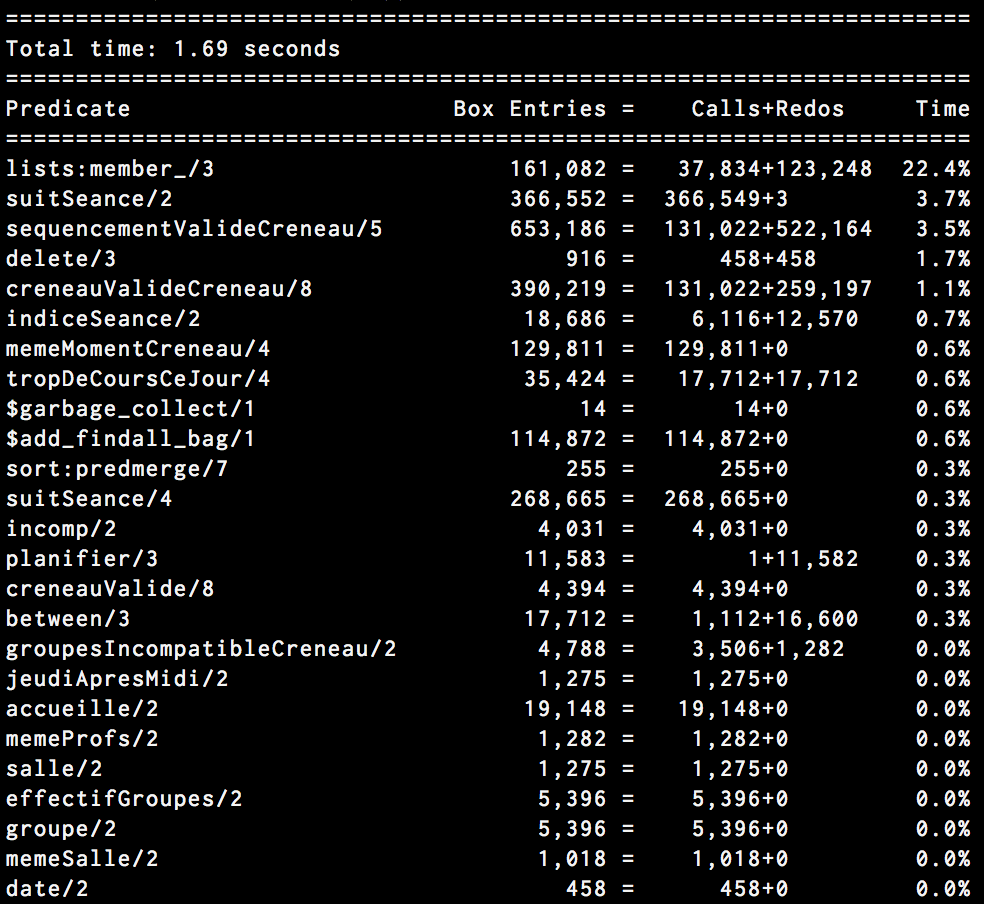
\includegraphics[keepaspectratio=true,width=12cm]{profile.png}
        \caption{\label{fig:profile} Résultat du profiling }
\end{figure}
